\section{Assembly and Validation of Processor 
(Assemblage et Validation du Processeur)}

\subsection{Assemble Processor}
\label{sec:Assemble Processor}

We modifying the modeling of the processor by assembling its three main units
\begin{itemize}
    \item The instruction management unit
    \item The processing unit
    \item The control unit
\end{itemize}

Complete the previously designed processing unit by adding a
2-input 4-bit multiplexer controlled by the RegSel control signal
generated by the control unit. This multiplexer will be placed at the input of the address
Rb of the register file, as shown in the Figure \ref{fig:AsmbUTf}.

\begin{figure}[htp]
    \centering
    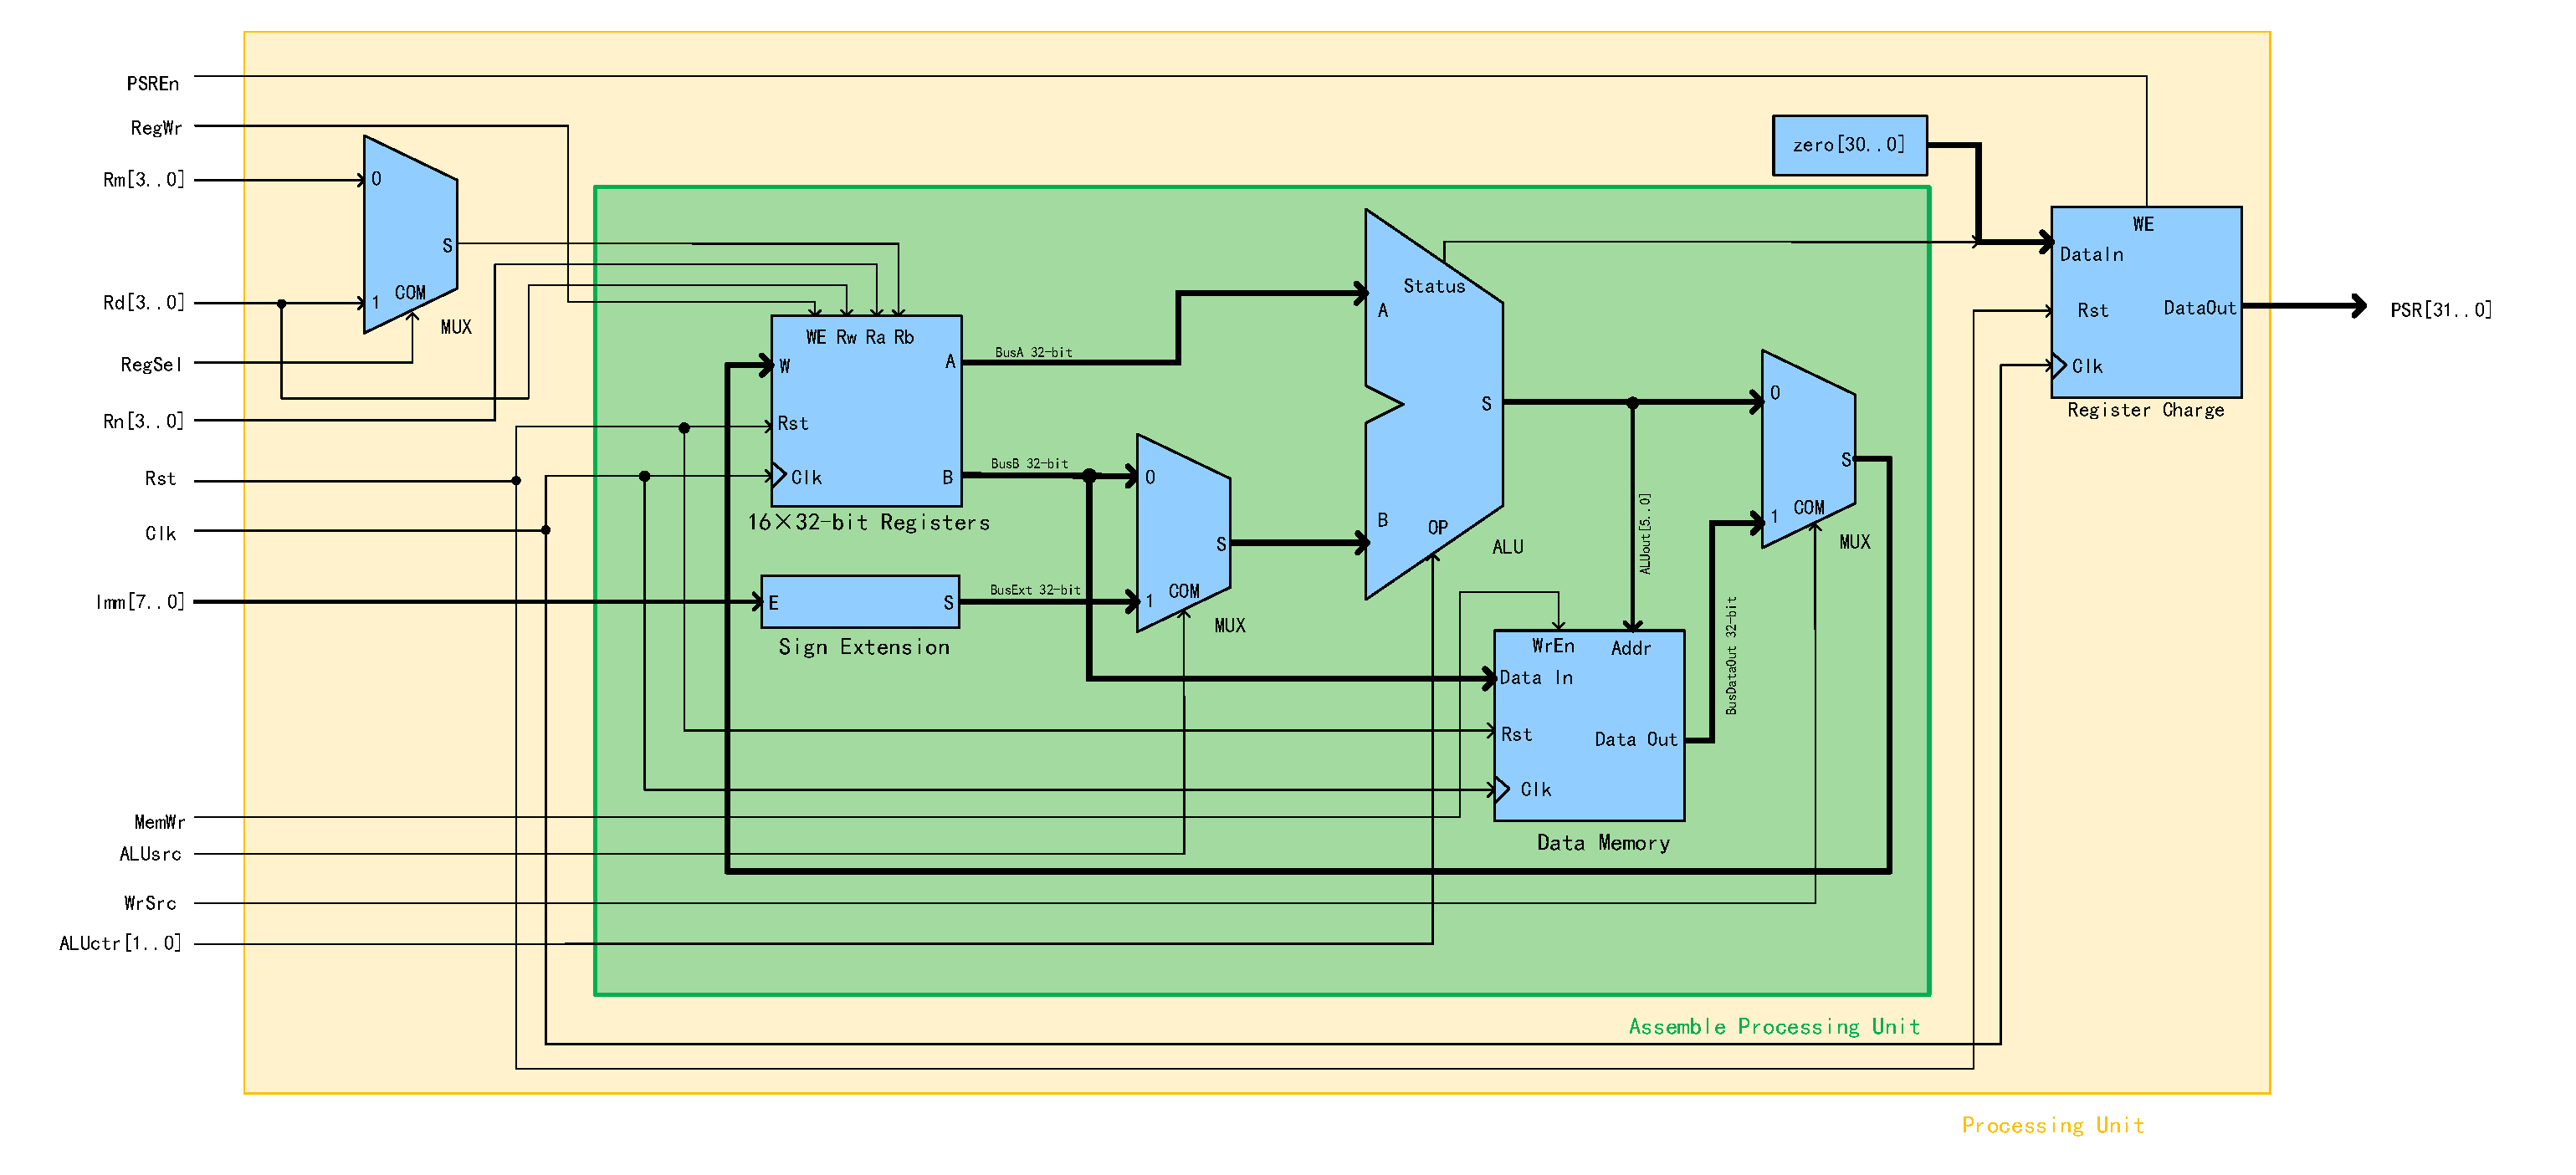
\includegraphics[width=1.5\textwidth, angle = 270]{picture/AsmbUTf.pdf}
    \caption{Processing Unit Block Diagram}     
    \label{fig:AsmbUTf}
\end{figure}

According to this block diagram, we modify the code for \textbf{Processing\_Unit.vhd}.

\begin{lstlisting}[style=vhdl, breaklines]
entity Processing_Unit is 
    port (
        clk, rst, MemWr, RegWr, ALUsrc, WrSrc ,RegSel, PSREn: in  std_logic ; 
        Rn, Rm, Rd : in std_logic_vector(3 downto 0);
        busout : out std_logic_vector(31 downto 0);--PSR[31..0]
        Imm : in std_logic_vector(7 downto 0); 
        ALUctr : in std_logic_vector(1 downto 0)
    );
end entity;
  
architecture behave of Processing_Unit is
    signal busA,busB,ALUS,busExtension,busMux, busW : std_logic_vector(31 downto 0);
    signal DataOut ,fl: std_logic_vector(31 downto 0);
    signal Rb : std_logic_vector(3 downto 0); 
    signal N: std_logic;
begin
  
    Register_File : entity work.Register_File port map(Clk => clk, rst => rst, WE=> RegWr, Ra => Rn, Rb => Rb, Rw => Rd, A => busA, B => busB, W=> busW); 
  
    ALU : entity work.ALU port map(A => busA, B=> busMux, S => ALUS, OP => ALUctr, N => N); 
  
    Sign_Extension : entity work.Sign_Extension port map ( E => Imm, S => busExtension);
  
    MUX1 : entity work.MUX port map (A => busB, B=> busExtension, S=> busMux, COM => ALUSrc); 
  
    MUX2 : entity work.MUX port map (A => ALUS, B=> DataOut, S=> busW, COM => WrSrc);
  
    Data_Memory : entity work.Data_Memory port map (Clk => clk, rst => rst, Addr => ALUS(5 downto 0), WE => MemWr, DataIn => busB, DataOut => DataOut); 
  
    MUX3 : entity work.MUX generic map( N=> 4) port map (A => Rm, B => Rd, COM => RegSel, S=> Rb); 
  
    Register_Charge : entity work.Register_Charge port map (clk => clk, rst => rst, WE => PSREn, DataIn => fl, DataOut => busout); 
  
    fl <= N&"000"&X"0000000";
  
end architecture;
\end{lstlisting}

With addition of \textbf{Processing\_Unit}, \textbf{Instruction\_Management\_Unit} and 
\textbf{Decoder}, the \textbf{Processor} can be assembled as Figure \ref{fig:PUs}. The detailed block diagram
will be given in the Appendices \ref{AppendicesA}.
\begin{figure}[htp]
    \centering
    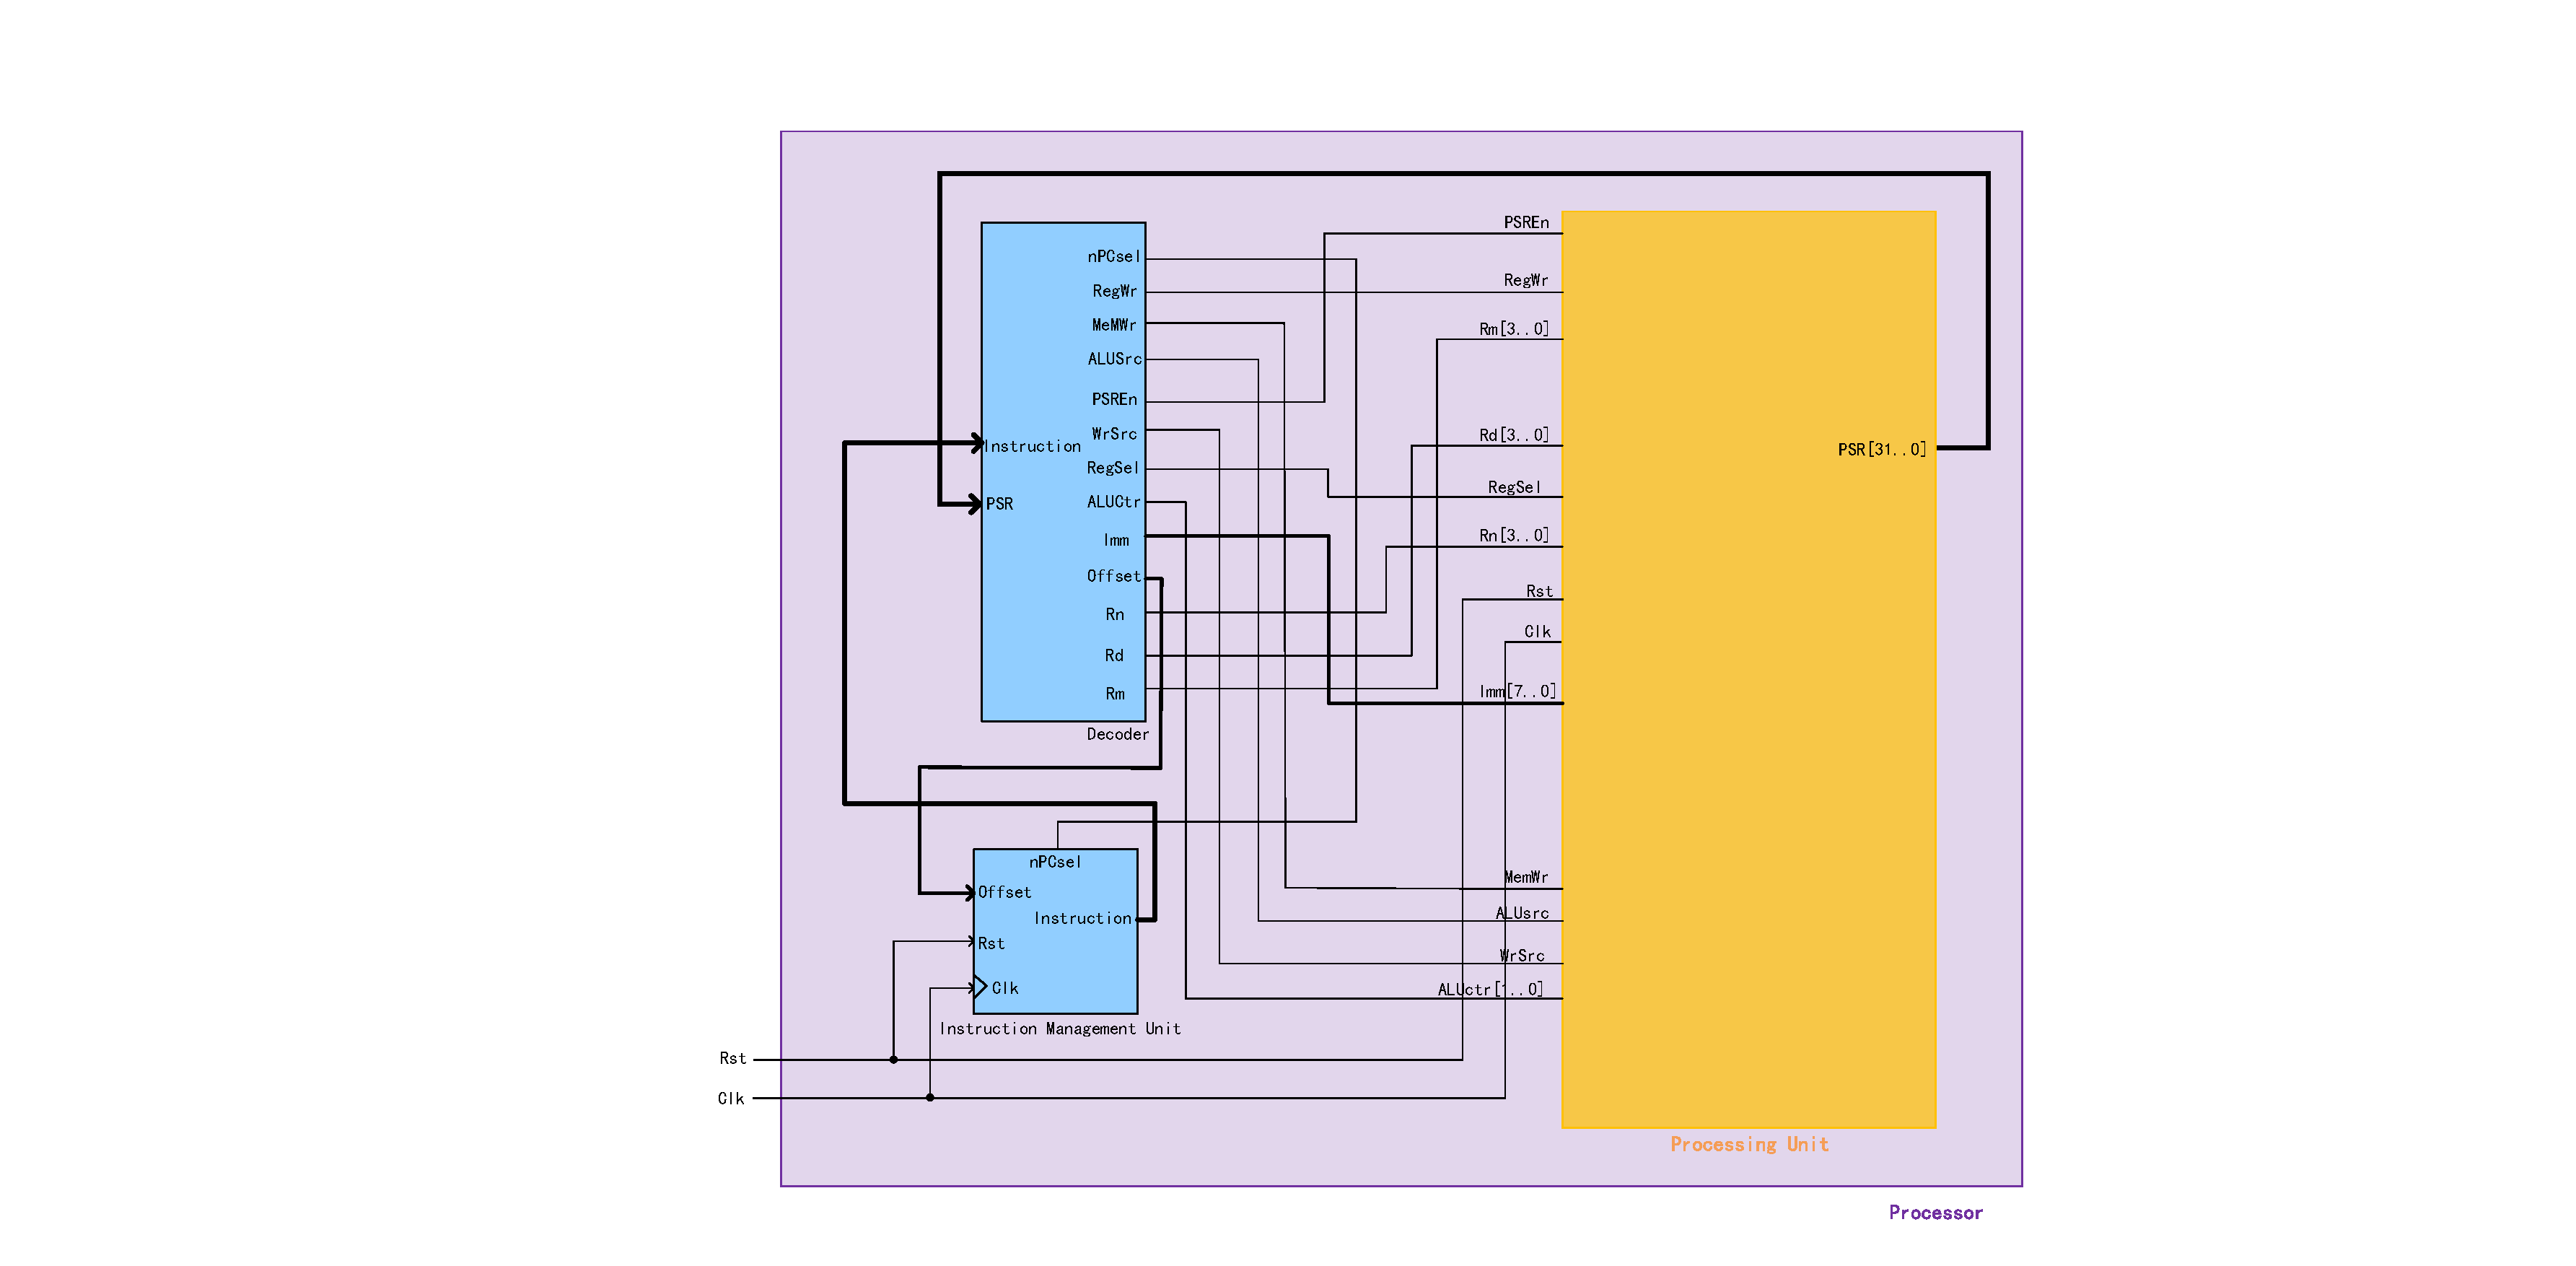
\includegraphics[width=1\textwidth]{picture/PUs.pdf}
    \caption{ProcessorBlock Diagram}     
    \label{fig:PUs}
\end{figure}

Thus, the core code for \textbf{Processor.vhd} is shown below.
\vspace*{1mm}
\begin{lstlisting}[style=vhdl,breaklines]
architecture behave of Processor is
    signal nPCSel, MemWr, RegWr, ALUsrc, WrSrc, RegSel, PSRen : std_logic ;
    signal ALUctr : std_logic_vector(1 downto 0);
    signal offset : std_logic_vector(23 downto 0);
    signal Immediate: std_logic_vector(7 downto 0);
    signal Instruction, busout : std_logic_vector(31 downto 0);--busout -> PSR
    signal Rn, Rd, Rm : std_logic_vector(3 downto 0); 
begin

    Processing_Unit : entity work.Processing_Unit port map(clk => clk, rst => rst, RegWr=> RegWr, Rn => Rn, Rd => Rd, Rm=> Rm, busout => busout, Imm => Immediate, ALUctr=> ALUctr, MemWr=> MemWr, ALUSrc=> ALUSrc,WrSrc=> WrSrc, RegSel=> RegSel, PSRen => PSRen); 

    Instruction_Management_Unit : entity work.Instruction_Management_Unit port map(Clk => clk, rst => rst, nPCSel=> nPCSel, Instruction=> Instruction, offset => offset); 

    Decoder  : entity work.Decoder  port map(RegWr=> RegWr, Rn => Rn, Rd => Rd, Rm=> Rm, psrout => busout, Immediate =>Immediate, ALUctr=> ALUctr, MemWr=> MemWr, ALUSrc=> ALUSrc, WrSrc=> WrSrc, RegSel=> RegSel, PSRen => PSRen, nPCSel=> nPCSel, Instruction=> Instruction, offset=> offset); 

end architecture;
\end{lstlisting}



\subsection{Simulate Processor}
\label{sec:Simulate Processor}

According to the testbench shown below, we run the simulation with command file \textbf{Processor\_test.do} and obtaine the waves as Figure \ref{fig:PUres}.
Detailed waves can be found as Figure \ref{fig:ModelSim_ processeur_tb(bench)} in Appendices \ref{AppendicesA}.
\begin{lstlisting}[style=vhdl]
library ieee;
use ieee.std_logic_1164.all;
use ieee.numeric_std.all;
    
entity Processor_tb is
end entity;
    
architecture test_bench of Processor_tb is
    signal clk, rst: std_logic;
    signal done : std_logic := '0';
    constant clk_period : time:= 10 ns;
begin
    
    UUT : entity work.Processor(behave)port map(clk => clk,rst => rst);

    rst <= '1', '0' after clk_period;
    
    clock : process is 
    begin
        if done = '0' then
            clk <= '0';
            wait for clk_period/2;
            clk <= '1';
            wait for clk_period/2;
        else
            wait;
        end if;
    end process;
    
    signal_gen : process is
    begin
        done <= '0';
        wait for clk_period*180;
        done <= '1';
        wait;
    end process;
        
end architecture;
\end{lstlisting}

\begin{figure}[htp]
    \centering
    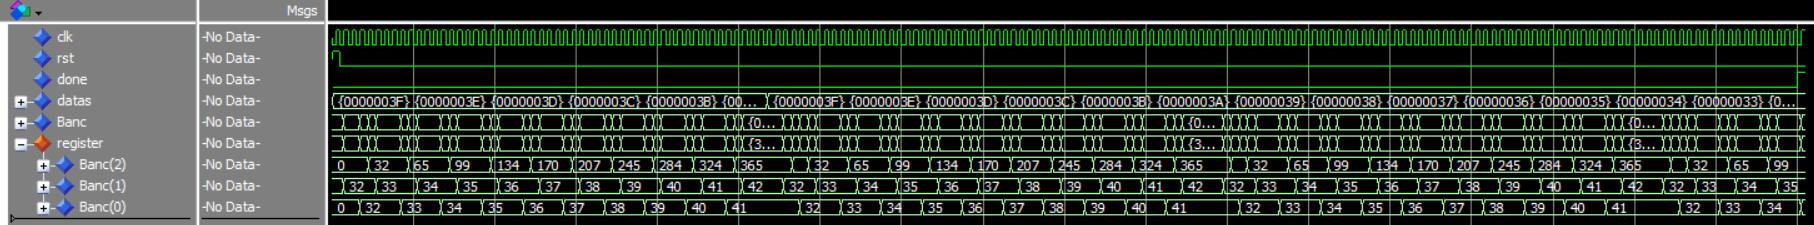
\includegraphics[width=1\textwidth]{picture/PUres.jpg}
    \caption{Simulation of Processing Unit}     
    \label{fig:PUres}
\end{figure}